\chapter{Descripci\'on del sistema}\label{ch:descripcion}

\begin{contenidoNuevo}

El presente cap\'itulo formaliza el an\'alisis funcional del prototipo construido para el hito del 50\,\%. Se documentan actores, historias de usuario, requerimientos funcionales y no funcionales, mockups de interfaz y el an\'alisis de competencias de mercado. El contenido se marca en azul para distinguir las incorporaciones respecto de la entrega del 25\,\%.

\section{Actores del sistema}

\begin{itemize}
	\item \textbf{Prevencionista:} consulta el riesgo de su zona, arma agenda y registra visitas.
	\item \textbf{Coordinador:} supervisa cobertura, indicadores y rebalanceo entre zonas.
	\item \textbf{Analista:} consulta m\'etricas del modelo y factores agregados (SHAP).
	\item \textbf{Administrador:} gestiona usuarios, roles y configuraci\'on b\'asica.
\end{itemize}

\section{Historias de usuario}

\begin{enumerate}
	\item \textbf{HU-01.} Como prevencionista, quiero autenticarme de forma segura para acceder solo a la informaci\'on de mi rol.
	\item \textbf{HU-02.} Como prevencionista, quiero ver un resumen operativo del d\'ia para saber qu\'e establecimientos cr\'iticos a\'un no tienen visita programada.
	\item \textbf{HU-03.} Como prevencionista, quiero priorizar establecimientos por horizonte mensual o trimestral para alinear urgencia y planificaci\'on.
	\item \textbf{HU-04.} Como prevencionista, quiero abrir el detalle de un establecimiento y entender por qu\'e est\'a priorizado, con explicaci\'on en lenguaje claro y factores SHAP.
	\item \textbf{HU-05.} Como prevencionista, quiero programar una visita desde la lista de riesgo o desde el detalle para convertir la predicci\'on en acci\'on.
	\item \textbf{HU-06.} Como prevencionista, quiero gestionar mi agenda (programadas, realizadas y canceladas) para cerrar el ciclo operativo.
	\item \textbf{HU-07.} Como coordinador, quiero ver estad\'isticas de cobertura y precisi\'on observada para evaluar el uso real del ranking.
	\item \textbf{HU-08.} Como coordinador, quiero exportar listados a CSV para compartir el plan de visitas fuera de la aplicaci\'on.
	\item \textbf{HU-09.} Como analista, quiero consultar factores SHAP agregados del top-50 y top-225 para validar coherencia del modelo.
	\item \textbf{HU-10.} Como administrador, quiero administrar usuarios y roles para controlar el acceso al prototipo.
	\item \textbf{HU-11.} Como usuario, quiero alternar tema claro/oscuro y colapsar el men\'u para trabajar con comodidad en jornadas largas.
	\item \textbf{HU-12.} Como coordinador, quiero distinguir motivos predictivos de obligaciones regulatorias (PRS) para no mezclar prioridades.
\end{enumerate}

\section{Requerimientos funcionales}

\begin{description}
	\item[RF-01 Autenticaci\'on] Login con usuario/contrase\~na, emisi\'on de JWT y cierre de sesi\'on con confirmaci\'on.
	\item[RF-02 Resumen operativo] Panel con estados de cobertura top-50/top-225 y accesos a priorizaci\'on/agenda.
	\item[RF-03 Priorizaci\'on] Listado de establecimientos ordenados por score, con filtros de horizonte (1m/3m), banda y b\'usqueda.
	\item[RF-04 Detalle] Ficha del establecimiento con score, banda, motivo, explicaci\'on de prioridad y factores SHAP individuales.
	\item[RF-05 Agenda] Alta, realizaci\'on y cancelaci\'on de visitas vinculadas al ranking vigente.
	\item[RF-06 Auditor\'ia operativa] Registro append-only de eventos del ciclo de visitas.
	\item[RF-07 Estad\'isticas] KPIs, cobertura hist\'orica, precisi\'on observada y SHAP agregado por cohorte.
	\item[RF-08 Exportaci\'on] Descarga CSV de listados relevantes para trabajo offline.
	\item[RF-09 Perfil] Consulta de datos de usuario y cambio de contrase\~na.
	\item[RF-10 Roles] Control de acceso por rol (Prevencionista, Coordinador, Analista, Admin).
	\item[RF-11 Snapshots] Consumo de rankings versionados e inmutables importados desde el pipeline.
	\item[RF-12 Doble horizonte] Soporte simult\'aneo de predicci\'on a 1 mes y a 3 meses.
\end{description}

\section{Requerimientos no funcionales}

\begin{description}
	\item[RNF-01 Seguridad] Autenticaci\'on JWT; contrase\~nas con hash; no exponer la BD core de la ART a Internet.
	\item[RNF-02 Desacople de datos] La aplicaci\'on opera sobre una BD propia (`PfiPrevencion`); el pipeline es el \'unico que lee la BD core on-prem.
	\item[RNF-03 Trazabilidad] Snapshots con hash de artefacto, vigencia y m\'etricas observadas auditables.
	\item[RNF-04 Usabilidad] Interfaz clara, paneles contextuales de ``c\'omo se calcula'', estados vac\'ios y confirmaciones.
	\item[RNF-05 Performance local] Respuesta interactiva en entorno local de demostraci\'on (API + web + SQL Express).
	\item[RNF-06 Explicabilidad] Las salidas del modelo se acompa\~nan de narrativa y SHAP; el score no se presenta como probabilidad.
	\item[RNF-07 Multi-ART] La arquitectura permite reutilizar la misma aplicaci\'on con distintas fuentes core de ART, sin acoplar nombres de proveedores.
	\item[RNF-08 Portabilidad cloud] Dise\~no compatible con despliegue futuro en AWS Free Tier (EC2 todo-en-uno), sin requerirlo para el hito 50\,\%.
\end{description}

\section{Diagrama de casos de uso}

La Figura~\ref{fig:casos-uso} resume las interacciones principales entre actores y el sistema.

\begin{figure}[htbp]
	\centering
	% Diagrama de casos de uso (UML 2: actor abstracto + generalizaci\'on)
\begin{tikzpicture}[
  font=\footnotesize\sffamily,
  uc/.style={
    ellipse,
    draw=NavyBlue!78,
    fill=white,
    minimum width=3.9cm,
    minimum height=0.86cm,
    align=center,
    inner sep=1.2pt,
    line width=0.8pt,
    font=\footnotesize\sffamily,
  },
  ucadm/.style={
    uc,
    draw=NavyBlue,
    fill=NavyBlue!10,
  },
  assoc/.style={line width=0.7pt, NavyBlue!65},
  gen/.style={
    line width=0.85pt,
    NavyBlue,
    -{Triangle[open, length=2.8mm, width=2.55mm]},
  },
  nametag/.style={
    font=\scriptsize\sffamily\bfseries,
    NavyBlue,
    fill=NavyBlue!6,
    rounded corners=3pt,
    inner sep=2.4pt,
    align=center,
  },
  stick/.pic={
    \fill[NavyBlue!18] (0,1.22) circle[radius=0.15];
    \draw[line width=0.82pt, NavyBlue]
      (0,1.22) circle[radius=0.15]
      (0,1.07) -- (0,0.50)
      (-0.28,0.90) -- (0.28,0.90)
      (0,0.50) -- (-0.22,0.10)
      (0,0.50) -- (0.22,0.10);
  },
]

  % Sombra de la tarjeta
  \fill[NavyBlue!11, rounded corners=8pt]
    (0.28,-4.78) rectangle (5.68,4.18);

  % Caja del sistema
  \path[rounded corners=8pt, fill=white, draw=NavyBlue!50, line width=0.95pt]
    (0.12,-4.62) rectangle (5.52,4.32);

  % Franja de t\'itulo
  \begin{scope}
    \clip[rounded corners=8pt] (0.12,-4.62) rectangle (5.52,4.32);
    \fill[NavyBlue!14] (0.12,3.66) rectangle (5.52,4.32);
  \end{scope}
  \draw[NavyBlue!50, line width=0.95pt] (0.12,3.66) -- (5.52,3.66);
  \node[font=\small\sffamily\bfseries, NavyBlue] at (2.82, 3.99)
    {Sistema Prevex};
  \draw[NavyBlue!50, line width=0.95pt, rounded corners=8pt]
    (0.12,-4.62) rectangle (5.52,4.32);

  % Casos compartidos
  \node[uc] (login)  at (2.82,  2.88) {Autenticarse};
  \node[uc] (riesgo) at (2.82,  1.82) {Priorizar visitas};
  \node[uc] (det)    at (2.82,  0.76) {Ver detalle (IA / SHAP)};
  \node[uc] (ag)     at (2.82, -0.30) {Gestionar agenda};
  \node[uc] (est)    at (2.82, -1.36) {Ver estad\'isticas};
  \node[uc] (perf)   at (2.82, -2.42) {Gestionar perfil};

  \draw[NavyBlue!30, dashed, line width=0.65pt]
    (0.42,-2.96) -- (5.22,-2.96);
  \node[font=\tiny\sffamily, NavyBlue!65, anchor=east] at (5.22, -3.16)
    {s\'olo administrador};

  \node[ucadm] (cfg) at (2.82, -3.84) {Administrar usuarios};

  % Actor abstracto
  \node[
    draw=NavyBlue,
    fill=NavyBlue!8,
    rounded corners=10pt,
    align=center,
    inner sep=6pt,
    line width=0.85pt,
    font=\scriptsize\sffamily,
    minimum width=2.15cm,
  ] (usr) at (-2.38, 0.95)
    {\textbf{Usuario}\\[-0.6pt]{\tiny autenticado}};

  % Actores concretos (m\'as aire vertical para que no se pisen las etiquetas)
  \pic at (-5.55, 2.28) {stick};
  \node[nametag, below, yshift=1pt] at (-5.55, 2.28) {Preventor};
  \coordinate (prev) at (-5.27, 3.18);

  \pic at (-5.55, 0.05) {stick};
  \node[nametag, below, yshift=1pt] at (-5.55, 0.05) {Coordinador};
  \coordinate (coord) at (-5.27, 0.95);

  \pic at (-5.55, -2.18) {stick};
  \node[nametag, below, yshift=1pt] at (-5.55, -2.18) {Administrador};
  \coordinate (admin) at (-5.27, -1.28);

  % Generalizaci\'on UML: un solo tri\'angulo hueco (sin flechas superpuestas)
  \coordinate (gjoin) at (-3.88, 0.95);
  \draw[line width=0.85pt, NavyBlue, rounded corners=2pt] (prev)  |- (gjoin);
  \draw[line width=0.85pt, NavyBlue] (coord) -- (gjoin);
  \draw[line width=0.85pt, NavyBlue, rounded corners=2pt] (admin) |- (gjoin);
  \draw[gen] (gjoin) -- (usr.west);

  % Asociaciones compartidas en ruteo ortogonal (sin abanico ni cruces)
  \coordinate (hub) at (-0.18, 0.95);
  \draw[assoc] (usr.east) -- (hub);
  \draw[assoc] (hub |- login.west) -- (hub |- perf.west);
  \foreach \u in {login, riesgo, det, ag, est, perf}
    \draw[assoc] (hub |- \u.west) -- (\u.west);

  % Administrar usuarios: baja desde el administrador y entra por debajo
  \draw[assoc, rounded corners=5pt]
    (admin) -- ++(0,-1.42) -| (cfg.west);

\end{tikzpicture}

	\caption{Diagrama de casos de uso del prototipo (hito 50\,\%).}
	\label{fig:casos-uso}
\end{figure}

\section{Mockups y dise\~no de interfaz}

El dise\~no previo se document\'o mediante wireframes de layout y mapa de pantallas. Luego se implement\'o el frontend React. La Figura~\ref{fig:wireframe-layout} muestra el esquema general; las Figuras~\ref{fig:mock-login}--\ref{fig:mock-estadisticas} ilustran las pantallas principales del prototipo.

\begin{figure}[htbp]
	\centering
	% Wireframe previo del layout global (análisis de diseño)
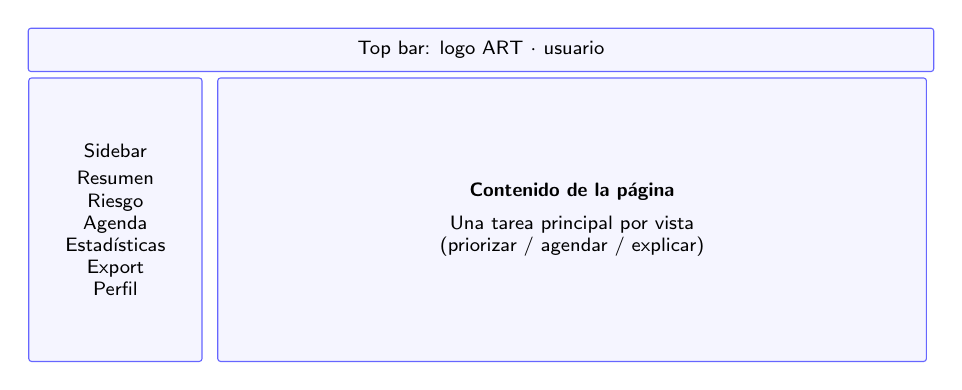
\begin{tikzpicture}[
  font=\scriptsize\sffamily,
  box/.style={draw=blue!60, fill=blue!4, rounded corners=1pt, align=center},
  ]
  \node[box, minimum width=11.5cm, minimum height=0.55cm] (top) at (0,3.2)
    {Top bar: logo ART $\cdot$ usuario};
  \node[box, minimum width=2.2cm, minimum height=3.6cm, anchor=north west] (side) at (-5.75,2.85)
    {Sidebar\\[2pt]Resumen\\Riesgo\\Agenda\\Estad\'isticas\\Export\\Perfil};
  \node[box, minimum width=9.0cm, minimum height=3.6cm, anchor=north west] (main) at (-3.35,2.85)
    {\textbf{Contenido de la p\'agina}\\[4pt]
     Una tarea principal por vista\\
     (priorizar / agendar / explicar)};
\end{tikzpicture}

	\caption{Wireframe del layout global (sidebar + top bar + contenido).}
	\label{fig:wireframe-layout}
\end{figure}

\begin{figure}[htbp]
	\centering
	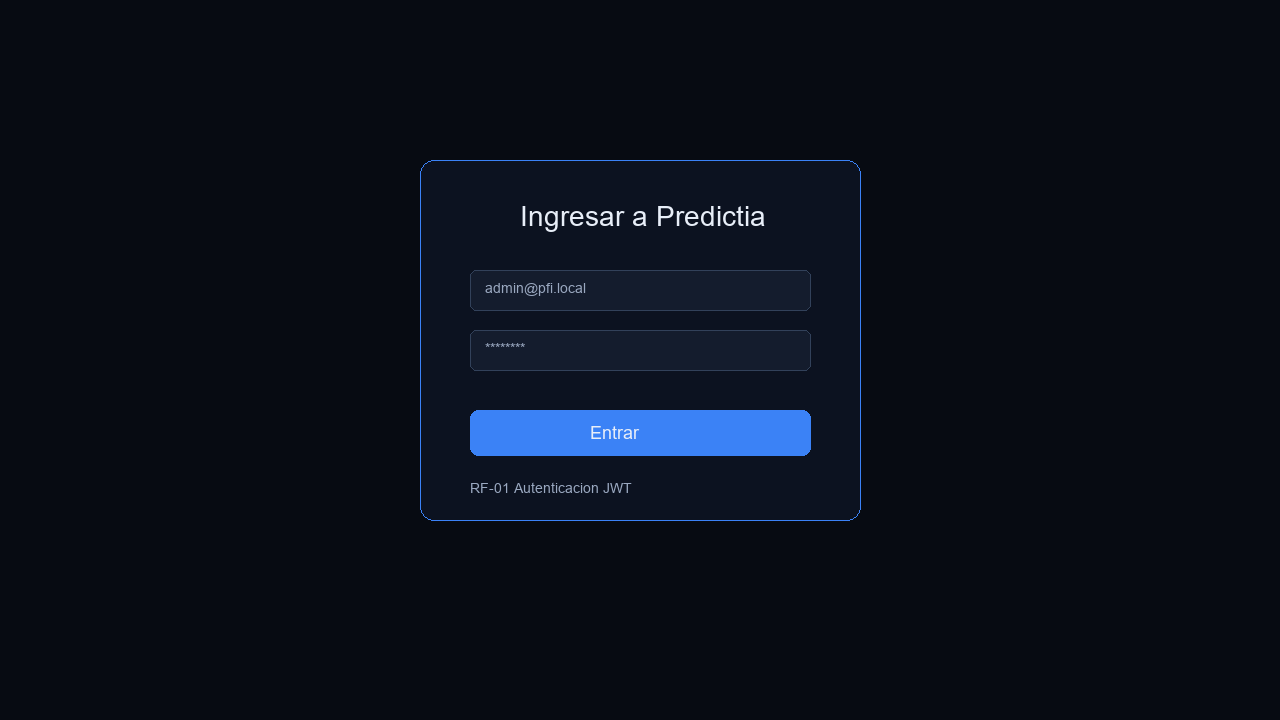
\includegraphics[width=0.92\textwidth]{figures/mockups/login.png}
	\caption{Mockup/pantalla de login (RF-01).}
	\label{fig:mock-login}
\end{figure}

\begin{figure}[htbp]
	\centering
	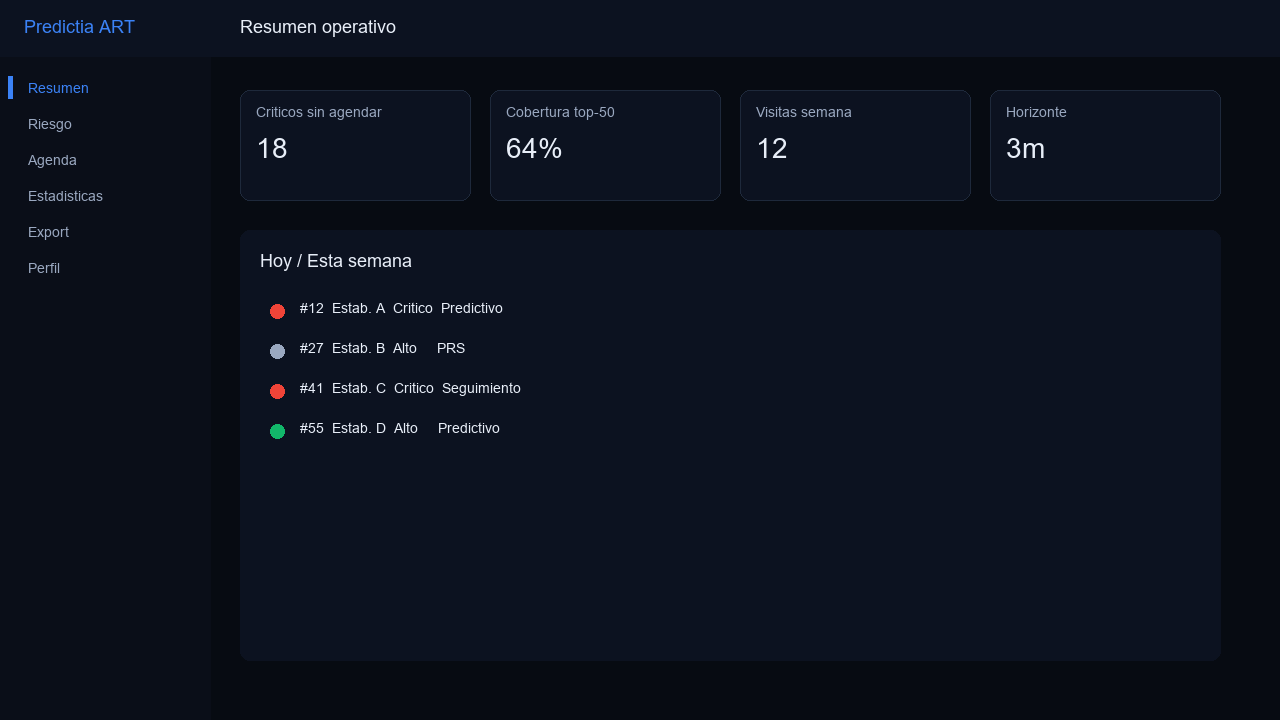
\includegraphics[width=0.92\textwidth]{figures/mockups/resumen.png}
	\caption{Pantalla de resumen operativo (RF-02 / HU-02).}
	\label{fig:mock-resumen}
\end{figure}

\begin{figure}[htbp]
	\centering
	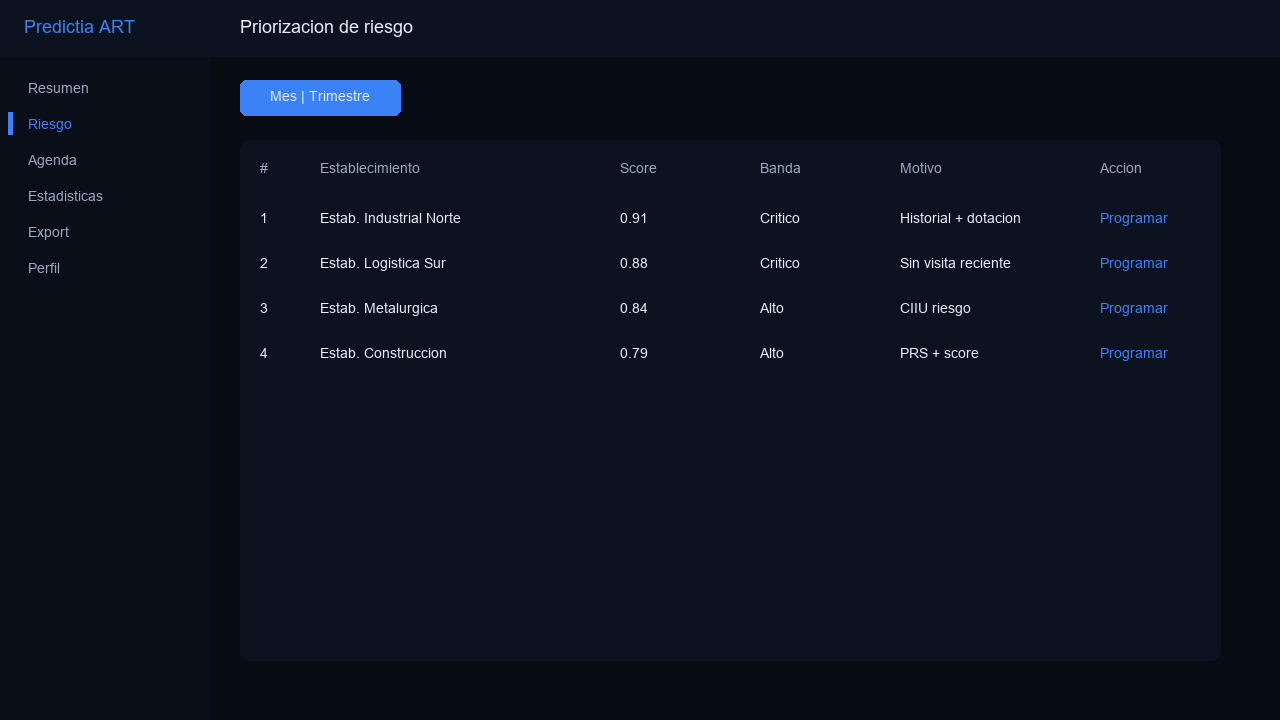
\includegraphics[width=0.92\textwidth]{figures/mockups/riesgo.png}
	\caption{Pantalla de priorizaci\'on de riesgo (RF-03 / HU-03).}
	\label{fig:mock-riesgo}
\end{figure}

\begin{figure}[htbp]
	\centering
	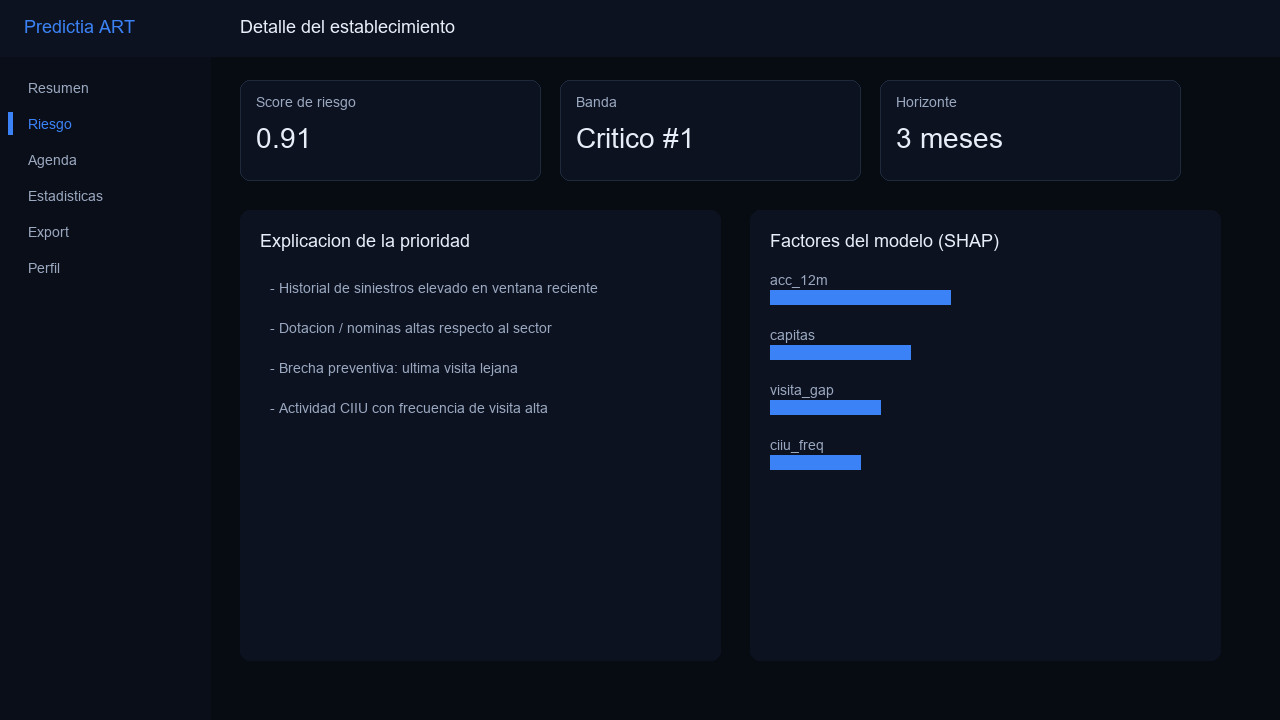
\includegraphics[width=0.92\textwidth]{figures/mockups/detalle.png}
	\caption{Detalle con explicaci\'on de prioridad y SHAP (RF-04 / HU-04).}
	\label{fig:mock-detalle}
\end{figure}

\begin{figure}[htbp]
	\centering
	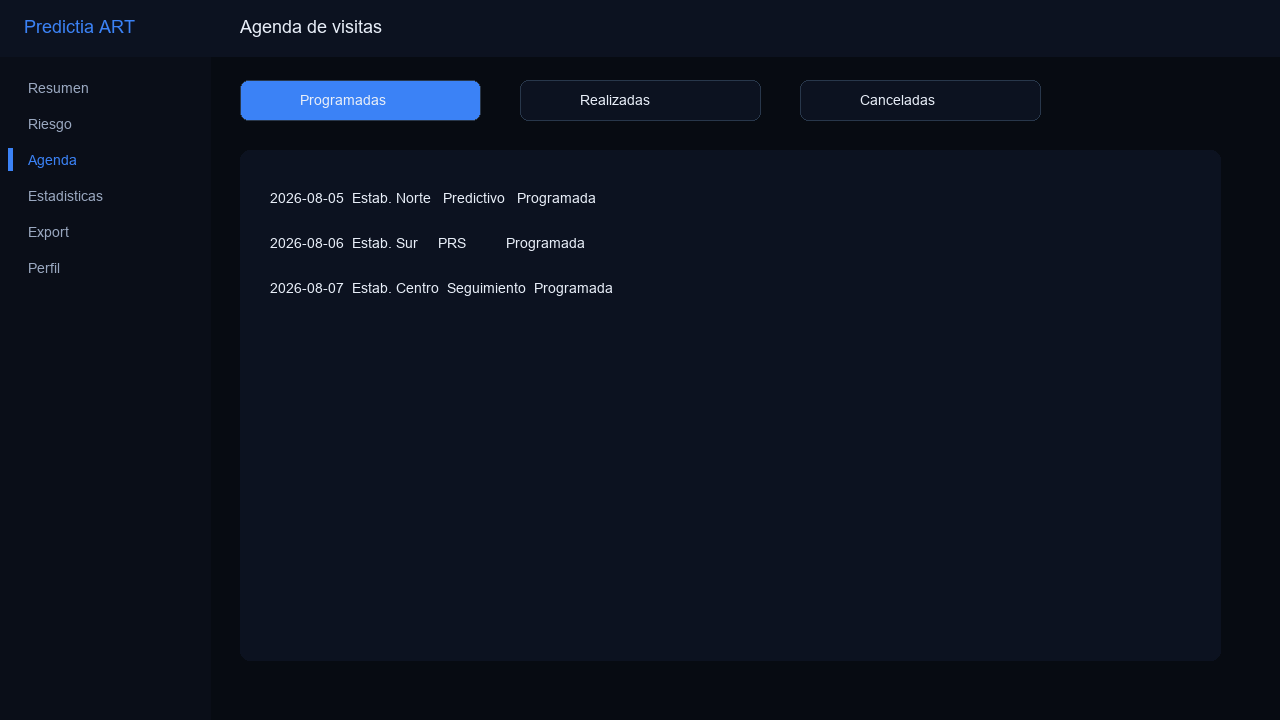
\includegraphics[width=0.92\textwidth]{figures/mockups/agenda.png}
	\caption{Agenda operativa de visitas (RF-05 / HU-06).}
	\label{fig:mock-agenda}
\end{figure}

\begin{figure}[htbp]
	\centering
	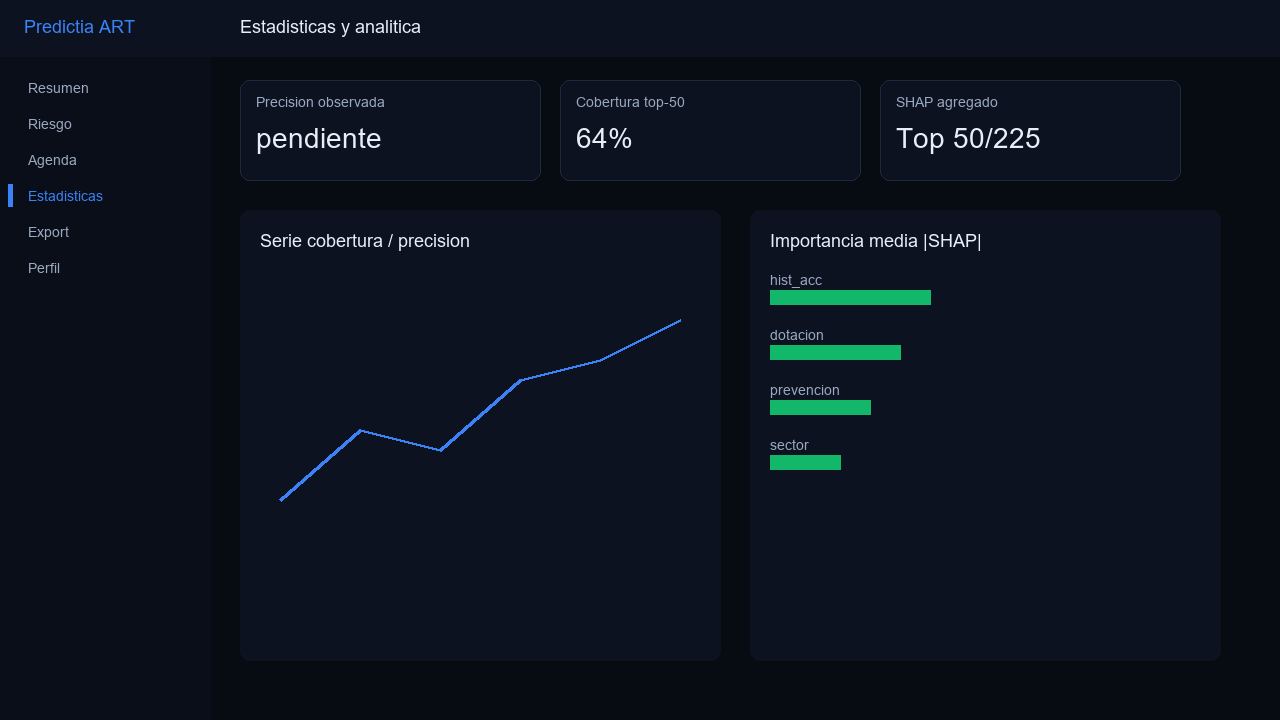
\includegraphics[width=0.92\textwidth]{figures/mockups/estadisticas.png}
	\caption{Estad\'isticas de cobertura, precisi\'on y SHAP agregado (RF-07 / HU-07).}
	\label{fig:mock-estadisticas}
\end{figure}

\section{An\'alisis de competencias}

\subsection{An\'alisis FODA}

\begin{table}[htbp]
	\centering
	\caption{An\'alisis FODA del sistema predictivo para ART.}
	\label{tab:foda}
	\begin{tabular}{@{}p{0.46\textwidth}p{0.46\textwidth}@{}}
		\hline
		\textbf{Fortalezas} & \textbf{Oportunidades} \\
		\hline
		Predicci\'on a nivel establecimiento con XGBoost validado en holdout 2025; explicabilidad SHAP accionable; app operativa (agenda + cobertura); desacople app/core ART. &
		Marco Prevenci\'on 4.0 y Res.\ SRT 48/2025; demanda de priorizaci\'on eficiente; escalabilidad multi-ART; despliegue cloud posterior. \\
		\hline
		\textbf{Debilidades} & \textbf{Amenazas} \\
		\hline
		User research a\'un pendiente; dependencia de calidad/completitud de datos hist\'oricos; prototipo a\'un no desplegado en nube. &
		Resistencia a modelos ``caja negra''; competencia de BI gen\'erico; cambios regulatorios; riesgo de malinterpretar el score como probabilidad. \\
		\hline
	\end{tabular}
\end{table}

\subsection{Fuerzas de Porter}

\begin{enumerate}
	\item \textbf{Rivalidad:} cores de seguros con reglas est\'aticas y plataformas BI gen\'ericas (alta capacidad t\'ecnica, baja especializaci\'on ART/prevenci\'on).
	\item \textbf{Nuevos entrantes:} startups de HSE analytics; barrera: acceso a datos reales de ART y encaje normativo local.
	\item \textbf{Poder de proveedores:} infraestructura cloud y librer\'ias ML est\'andar; riesgo bajo por uso de stack abierto (.NET, React, XGBoost).
	\item \textbf{Poder de clientes (ART):} alto; exigen trazabilidad, seguridad y utilidad para prevencionistas de campo.
	\item \textbf{Sustitutos:} ranking manual por CIIU/PESE, planillas y criterios expertos sin modelo.
\end{enumerate}

El diferencial del proyecto es combinar predicci\'on prospectiva, XAI y flujo operativo (agenda/cobertura) en una interfaz pensada para el prevencionista, no solo para el cient\'ifico de datos.

\subsection{Triple P (Producto--Precio--Plaza)}

\begin{description}
	\item[Producto] Sistema de priorizaci\'on predictiva de visitas con explicabilidad y gesti\'on operativa (agenda, auditor\'ia, indicadores).
	\item[Precio] Modelo de valor orientado a eficiencia de panel (mejor precisi\'on top-K vs.\ visitas reales) m\'as que a licencia gen\'erica de BI; en la tesis el prototipo se valida sin comercializaci\'on.
	\item[Plaza] Canal directo a equipos de prevenci\'on de ART (intranet/demo local hoy; cloud Free Tier/EC2 como arquitectura objetivo multi-ART).
\end{description}

\end{contenidoNuevo}
